\section{A Taxonomy of Inter-Agent Protocols}
\label{sec:taxonomy}

The remainder of the survey rests on a single structural claim:
the protocols of the 2024 to 2026 wave fall into \emph{three
architectural layers} of inter-agent coordination, distinguished
not by the technologies they use but by the question they
answer. Section~\ref{sec:taxonomy:layers} introduces the three
layers and the question each addresses. Section~\ref{sec:taxonomy:orthogonal}
identifies three orthogonal classification axes that cut across
the layer assignment. Section~\ref{sec:taxonomy:tree} renders the
resulting taxonomy as Figure~\ref{fig:taxonomy}.
Section~\ref{sec:taxonomy:complementary} closes by arguing that
the most-discussed apparent rivalry in the literature
(MCP versus A2A) is in fact a layer confusion and that the
two protocols are complementary.

Other taxonomies of this space classify by system shape
rather than by protocol layer. The hierarchical-multi-agent
taxonomy of Moore~\cite{hierarchical_taxonomy} sorts systems
by coordination pattern: supervisor trees, peer pools, and
the industrial patterns built from them. That axis is
orthogonal to ours. A supervisor tree and a peer pool can
both run on A2A. The layer a protocol occupies does not tell
you the topology deployed on it. We classify what a
specification answers, because that is what the rubric of
\S\ref{sec:rubric} then scores.

\subsection{Three layers of inter-agent coordination}
\label{sec:taxonomy:layers}

\paragraph{Layer 1: Tool binding.}
The tool-binding layer answers the question \emph{how does
an agent invoke an external capability and consume its
result?} It is the layer at which a single agent, typically
an LLM, extends itself with external functions, data
sources, or sub-agents that the protocol presents
uniformly as tools. The defining structural feature is an
asymmetric, two-party call: an agent (the client) sends a
request to a capability provider (the server) and receives
either a synchronous result or a streaming continuation.
The Model Context Protocol is the canonical tool-binding
specification of the period~\cite{spec_mcp}; the IBM/BeeAI
ACP protocol~\cite{spec_acp} occupies the same layer with
different transport choices. Section~\ref{sec:industry-protocols}
treats this layer in depth.

\paragraph{Layer 2: Peer messaging.}
The peer-messaging layer answers the question \emph{how do
two or more agents, each capable of independent action and
each potentially long-lived, coordinate over a shared task?}
The defining structural feature is symmetric in two senses:
either party can initiate, and the conversation is
typically modeled as a stateful interaction that outlives
any single request. A2A is the most widely adopted peer-messaging
protocol~\cite{spec_a2a}; ANP, AGNTCY/SLIM, Coral, LOKA, and
ACNBP also occupy this layer with markedly different design
choices on identity (centralized OAuth versus DID), discovery
(registry-mediated versus peer-resolved), and async semantics
(push notifications versus checkpointing). Section~\ref{sec:emerging-protocols}
treats the non-A2A members of this layer.

\paragraph{Layer 3: Commerce settlement.}
The commerce-settlement layer answers a question that did
not have to be answered before agents began transacting on
behalf of human principals: \emph{how does an agent prove,
at the moment of payment, that it is acting within the
authority granted by its principal, and how is that
authority cryptographically traceable through the chain of
delegation?} The defining structural feature is the
\emph{intent-mandate-receipt envelope}: the agent's intended
action, the principal's signed mandate authorizing that
action class, and the cryptographically attested receipt
of execution form a tamper-evident chain that survives the
underlying payment rail. AP2~\cite{spec_ap2}, Visa
TAP~\cite{spec_visa_tap}, Mastercard Agent Pay, and
ERC-8004~\cite{spec_erc8004} are the four occupants of this
layer that carry the envelope. UCP~\cite{spec_ucp} is a fifth
occupant of a different kind: it specifies the commerce
transaction around the payment and consumes AP2's mandate
through an optional extension, so it carries no settlement
substrate of its own (\S\ref{sec:emerging:commerce}).
Section~\ref{sec:industry-protocols}
treats the commerce stack alongside the industry-led
peer-messaging protocols, since the same vendors govern
both layers in practice.

The three layers compose: a production multi-agent deployment
will typically use MCP for tool binding within each agent, A2A
or a peer-messaging counterpart for inter-agent task
delegation, and (where transactions are involved) AP2 or Visa
TAP for commerce-settlement attestation. The layers are not
substitutes; the most common conceptual error in the
contemporary literature is treating them as if they were.

\subsection{Orthogonal classification axes}
\label{sec:taxonomy:orthogonal}

Three classification axes cut across the layer assignment.
Each is binary or near-binary; together they suffice to
identify any given protocol uniquely.

\paragraph{Open versus consortium-governed.}
A protocol's governance shapes its survival prospects far
more than its technical design. We distinguish protocols
under named-individual or single-vendor authorship (LOKA,
ACNBP, the 2025 ANP white paper drafts) from those under a
formal standards-development organization or foundation
(A2A and MCP under the Linux Foundation Agentic AI
Foundation~\cite{lf_aaif}; ANP and AGNTCY trending toward
W3C and Linux Foundation respectively;
ERC-8004 within the Ethereum Improvement Proposal
process~\cite{spec_erc8004}). Governance is the subject of
the third sub-axis of Axis 10 in the rubric (\S\ref{sec:rubric})
and is treated independently in \S\ref{sec:governance}.

\paragraph{Registry-based versus peer-discovery.}
Protocols differ on how an agent finds another agent. A
registry-based protocol presumes a directory service through
which agents publish their existence and capabilities and
through which clients look them up; A2A's
\texttt{/.well-known/agent-card.json} convention is a
lightweight variant~\cite{spec_a2a}, and ACNBP's ANS
service~\cite{spec_acnbp} is a more elaborate one. A
peer-discovery protocol presumes that agents resolve each
other directly through identifiers, typically DIDs,
that carry their location and verification metadata; ANP and
LOKA are the canonical examples~\cite{spec_anp, spec_loka}.
The choice has direct consequences for Axes 1 and 2 of the
rubric.

\paragraph{Synchronous versus async-first.}
A protocol may treat synchronous request-response as the
primary pattern and add async semantics as an extension, or
it may treat the long-running task as the primary unit and
add synchronous shortcuts. MCP is synchronous-first; A2A is
async-first at the task level even though individual
messages are synchronous; ACNBP's ten-step capability
negotiation~\cite{spec_acnbp} is async-first by design.
Axis 6 of the rubric captures this distinction.

\subsection{The taxonomy tree}
\label{sec:taxonomy:tree}

Figure~\ref{fig:taxonomy} renders the resulting taxonomy.
The three architectural layers form the first split. Within
each layer, the orthogonal classification axes generate the
sub-tree. The thirteen protocols of the survey appear as
leaves; the leaf label carries the protocol identifier and
the rubric-summary triple (governance class, discovery
style, async style) that disambiguates its position from
its layer siblings.

\begin{figure*}
  \centering
  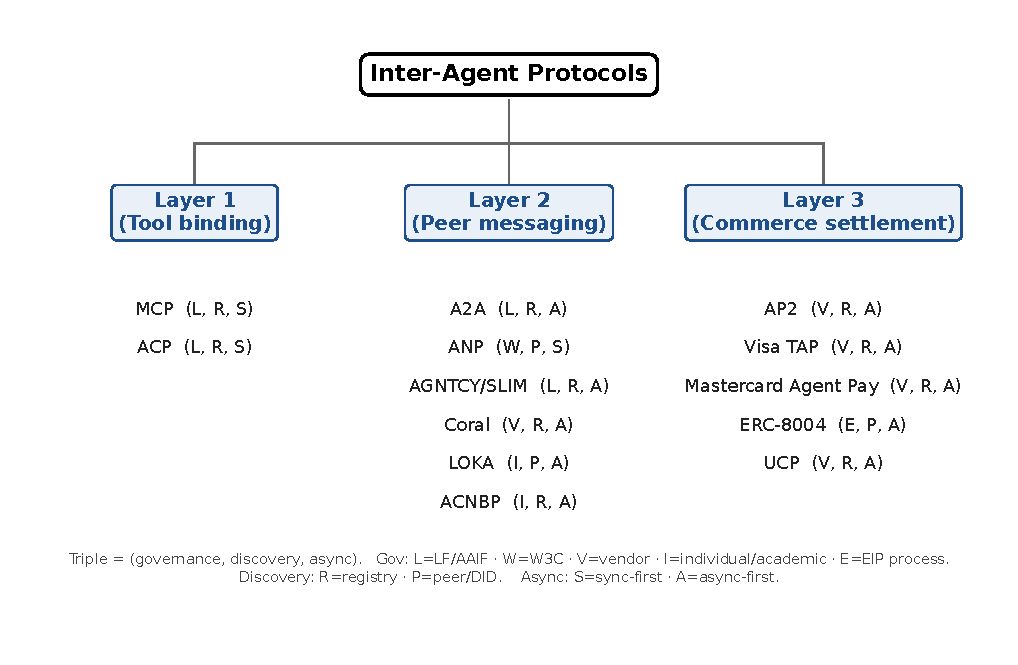
\includegraphics[width=\textwidth]{figures/fig-taxonomy.pdf}
  \caption{Three-layer taxonomy of the thirteen protocols
  surveyed. Layer assignment is by the coordination
  question the protocol answers, not by technology choice.
  Each leaf carries the orthogonal-axes triple
  (governance, discovery, async) introduced earlier in
  this section.}
  \label{fig:taxonomy}
\end{figure*}

\subsection{Why MCP and A2A are complementary, not competitive}
\label{sec:taxonomy:complementary}

The most-discussed apparent rivalry in the contemporary
literature is between MCP and A2A. Vendors and commentators
have repeatedly framed the choice as a binary: \emph{do we
ship MCP or A2A?} The framing is a category error, and
clarifying it is the single most useful corrective the
taxonomy contributes.

MCP is a tool-binding protocol. Its design answers the
question \emph{how does an agent invoke external
capabilities?} The asymmetric client-server shape, the
JSON-Schema input contracts, the streaming-result
extension, and the OAuth-2.1 transport security model are
all coherent answers to that question. MCP does not
specify how two long-lived agents coordinate; it does not
need to.

A2A is a peer-messaging protocol. Its design answers the
question \emph{how do two agents coordinate over a
long-lived task?} The Task lifecycle, the Parts and
Artifacts content model, the AgentCard discovery
convention, and the push-notification async pattern are
all coherent answers to that question. A2A does not
specify how a single agent extends itself with external
tools; it does not need to.

A production multi-agent deployment with both kinds of
coordination will typically run MCP \emph{inside} each
A2A agent, with MCP servers providing the agent's
tool-binding layer and A2A providing the inter-agent
coordination layer above. The two protocols are designed
to compose. Several emerging frameworks, including
Coral~\cite{spec_coral}, explicitly assume this
composition: Coral's tool integration is MCP-mediated
while its inter-agent threads are peer-messaging at a
different layer.

The same composition extends to the commerce-settlement
layer: where an A2A agent acts on behalf of a human
principal in a transaction, AP2 or Visa TAP carries the
intent-mandate-receipt chain alongside the A2A task,
without either protocol needing to absorb the other's
concerns. The three-layer taxonomy is, in this sense, not
merely descriptive; it is the assumption that lets the
protocols of the period \emph{compose} rather than
\emph{conflict}.
